
\begin{figure*}[h]
%	\captionsetup[subfigure]{}
	\begin{center}
		
		\begin{subfigure}{.49\linewidth}
			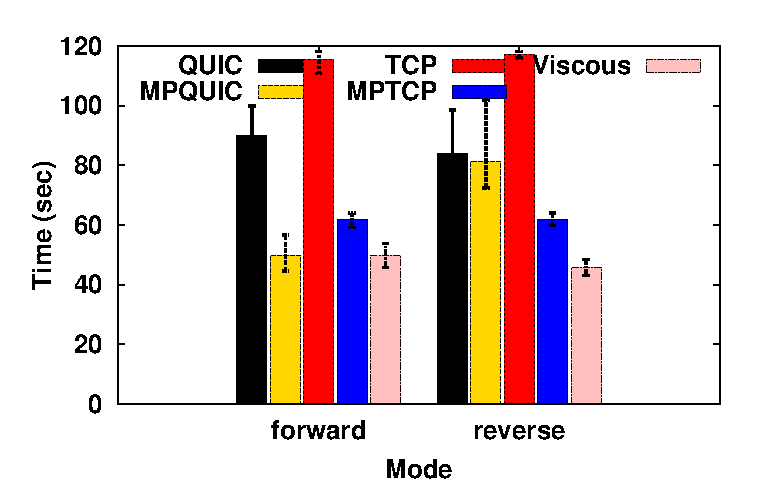
\includegraphics[width=0.95\linewidth]{img/rocketfuel/tymdiff-5-5.eps}
			\caption{\label{fig:rocketfuel_time_5_20}Delay=5ms \#threads=5}
		\end{subfigure}
		\begin{subfigure}{.49\linewidth}
			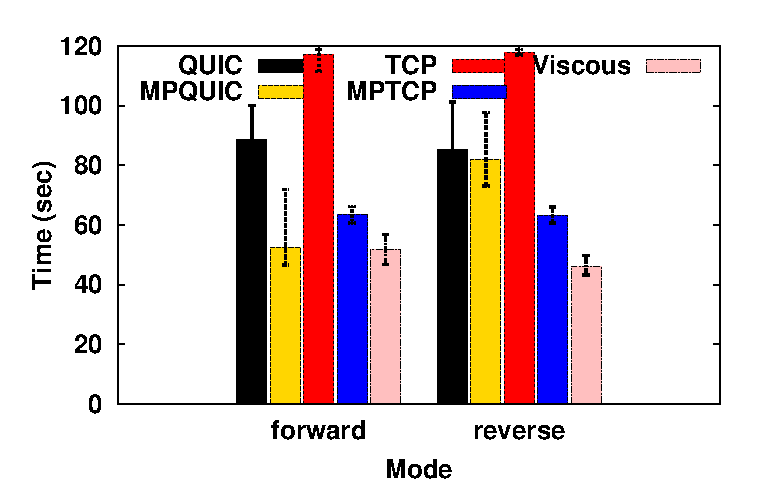
\includegraphics[width=0.95\linewidth]{img/rocketfuel/tymdiff-10-5.eps}
			\caption{\label{fig:rocketfuel_time_10_5}Delay=10ms \#threads=5}
		\end{subfigure}
		\begin{subfigure}{.49\linewidth}
			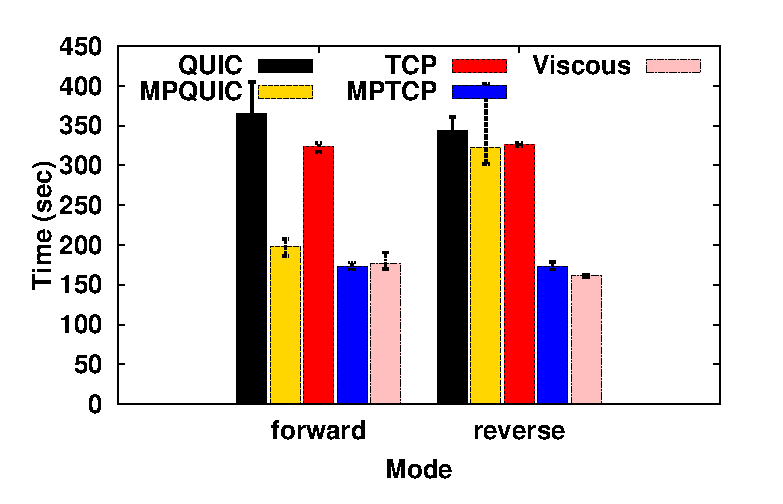
\includegraphics[width=0.95\linewidth]{img/rocketfuel/tymdiff-10-20.eps}
			\caption{\label{fig:rocketfuel_time_10_20}Delay=10ms \#threads=20}
		\end{subfigure}
		\begin{subfigure}{.49\linewidth}
			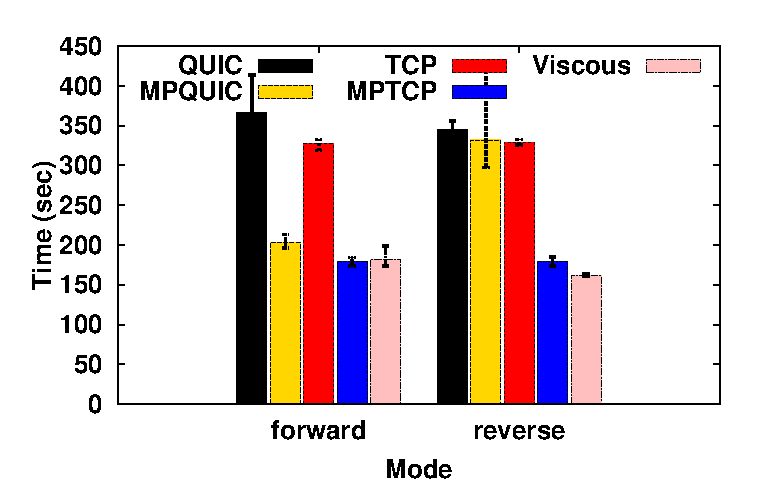
\includegraphics[width=0.95\linewidth]{img/rocketfuel/tymdiff-20-20.eps}
			\caption{\label{fig:rocketfuel_time_20_20}Delay=20ms \#threads=20}
		\end{subfigure}
		\caption{\label{fig:rocketfuel_time}Average average flow completion time over Rocketfuel topology}
	\end{center}
\end{figure*}


\begin{figure*}[h]
	\captionsetup[subfigure]{}
	\begin{center}
		\begin{subfigure}{.49\linewidth}
			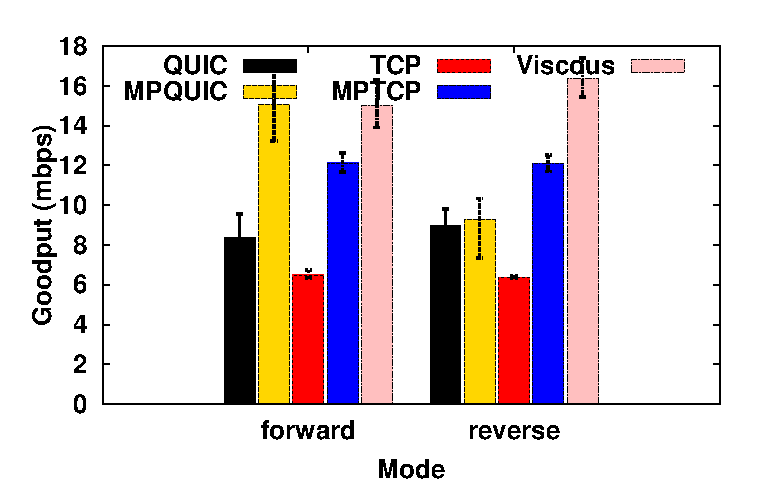
\includegraphics[width=0.95\linewidth]{img/rocketfuel/goodPut-5-5.eps}
		 \caption{\label{fig:rocketfuel_goodput_5_20}Delay=5ms \#threads=5}
		\end{subfigure}
		\begin{subfigure}{.49\linewidth}
			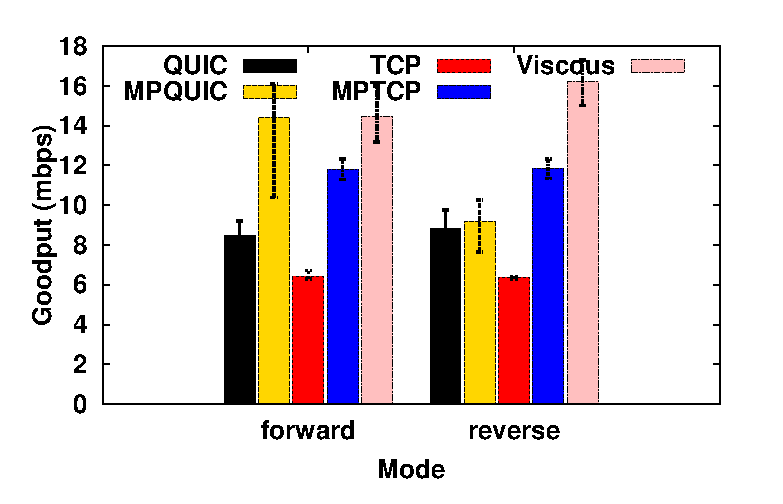
\includegraphics[width=0.95\linewidth]{img/rocketfuel/goodPut-10-5.eps}
		 \caption{\label{fig:rocketfuel_goodput_10_5}Delay=10ms \#threads=5}
		\end{subfigure}
		\begin{subfigure}{.49\linewidth}
			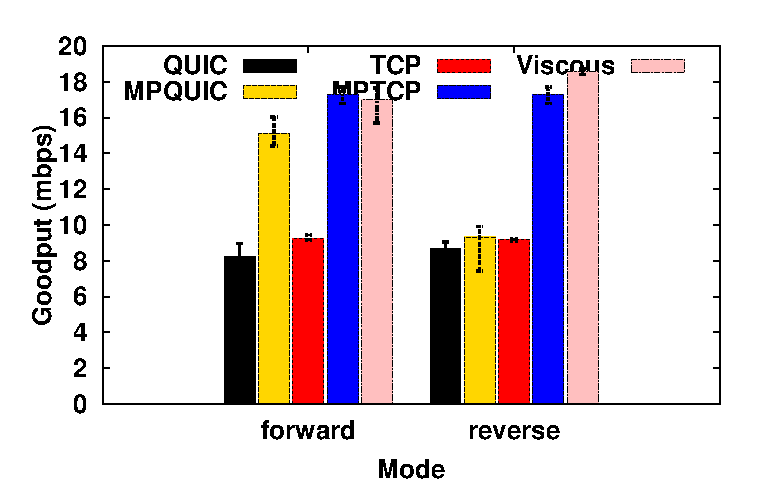
\includegraphics[width=0.95\linewidth]{img/rocketfuel/goodPut-10-20.eps}
		 \caption{\label{fig:rocketfuel_goodput_10_20}Delay=10ms \#threads=20}
		\end{subfigure}
		\begin{subfigure}{.49\linewidth}
			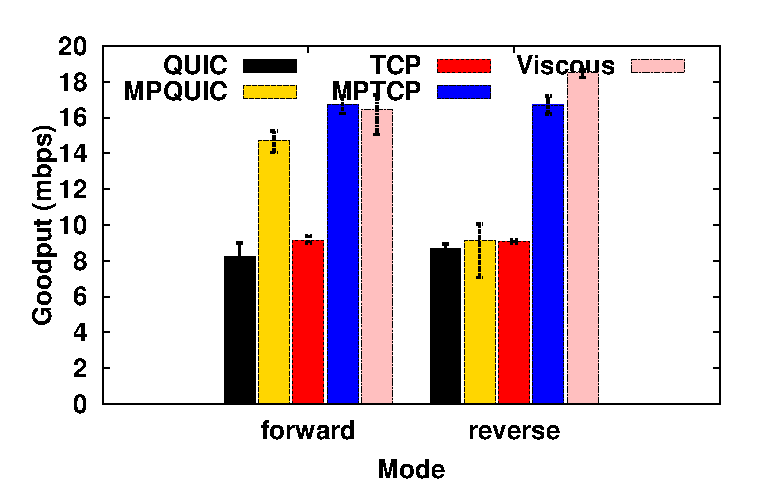
\includegraphics[width=0.95\linewidth]{img/rocketfuel/goodPut-20-20.eps}
		 \caption{\label{fig:rocketfuel_goodput_20_20}Delay=20ms \#threads=20}
		\end{subfigure}
		\caption{\label{fig:rocketfuel_goodput}Average GoodPut over Rocketfuel topology}
	\end{center}
\end{figure*}
\section{Results}
Previous section we have describe the different experimental setup. In this section, we analyze the results of those experiments.

\subsection{Overall performance}
We have describe the experimental setup in the section \ref{expsetup-rocketfuel}.
In Fig.~\ref{fig:rocketfuel_time} and Fig.~\ref{fig:rocketfuel_goodput}, we have shown few selected results. There are two observation we can get from these plot. Firstly, in all of the cases, Viscous performs as good as the MPQUIC. In fact, Viscous out performed MPQUIC in reverse flow experiment. It is happening because Viscous is true multi-path-multi-stream protocol, while QUIC is not a multi-path protocol. MPTCP is not a multi-stream protocol, so it required new connection for each transmission. MPQUIC is multi-path multi-stream protocol, but it suffers for reverse flow because, it can not take advantage of multiple interface during sending a datagram due the UDP api limitation. Viscous does not suffers in the reverse flow experiments because the Viscous use Packet-Socket api.



\subsection{Aggregated Benefit Measurement}

\begin{figure}
	\captionsetup[subfigure]{}
	\begin{center}
		\begin{subfigure}{.49\linewidth}
			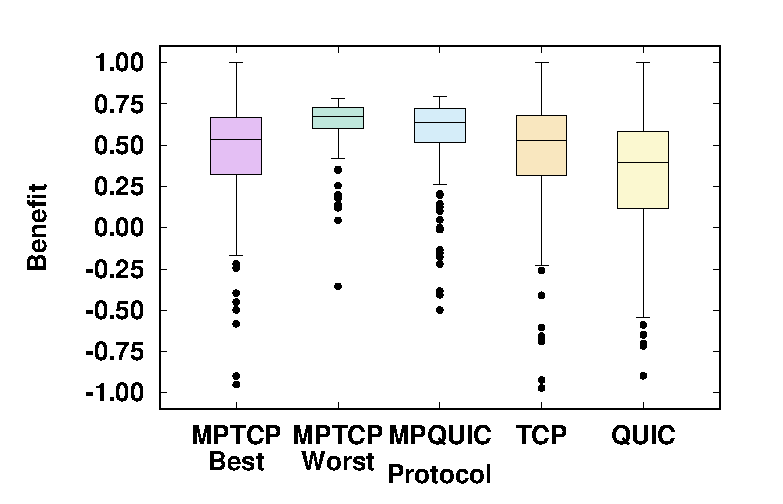
\includegraphics[width=.95\linewidth]{img/lowbdp-lossless/lowbdpnoloss_benefit.eps}
		 \caption{\label{fig:benefit-box} Benefit of Viscous over other transport different protocol}
		\end{subfigure}
		\begin{subfigure}{.49\linewidth}
			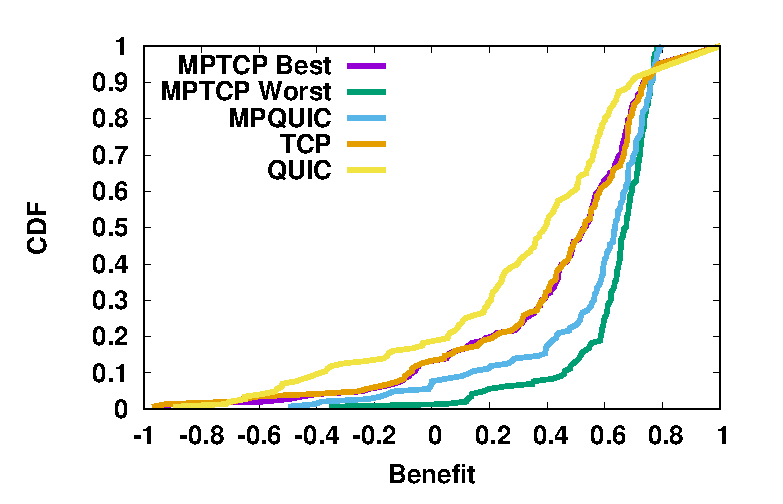
\includegraphics[width=.95\linewidth]{img/lowbdp-lossless/lowbdpnoloss_cdf.eps}				 
		 \caption{\label{fig:benefit-cdf} CDF of benefit of Viscous over other transport different protocol}
		\end{subfigure}
		\caption{\label{fig:benefit}Experimental results on lossless low BDP channels}
	\end{center}
\end{figure}

In Fig.~\ref{fig:benefit}, \ref{fig:benefit-high}, \ref{fig:benefit-lossy} and \ref{fig:benefit-high-lossy}, we have depicted the result of our experiment on aggregated benefit of Viscous.
We can see that the Viscous is performing better than all the other protocols in all the scenarios. It can be understood that, the TCP and the MPTCP aren't performing good enough because they need to go through slow-start phase for every request. A loss of a packet during slow start state can reduce throughput of TCP and MPTCP greatly as it causes unsaturated reduction of the $cwnd$. However QUIC and MP-QUIC should not have such problem as they uses multiple types of signal to understand congestion. So, after taking close look to we found that QUIC and MP-QUIC have strict flow control mechanism at connection level to by setting receivers' window size to 3.5MB. This flow control causing the reduction of the speed for the QUIC and MP-QUIC while the Bandwidth or the RTT of the link is little higher (i.e. BDP is higher that $3.5$ MB). However, Viscous do not have such connection level flow control. It have flow control only at the flow layer. So, Viscous is performing better even in case of lossy channel.

\begin{figure}
	\captionsetup[subfigure]{}
	\begin{center}
		\begin{subfigure}{.49\linewidth}
			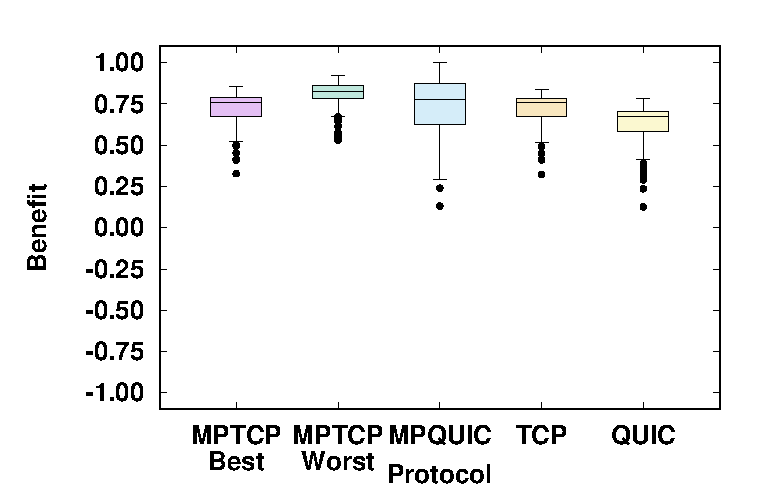
\includegraphics[width=.95\linewidth]{img/highbdp-lossless/highbdpnoloss_benefit.eps}
		 \caption{\label{fig:benefit-box-high} Benefit of Viscous over other transport different protocol}
		\end{subfigure}
		\begin{subfigure}{.49\linewidth}
			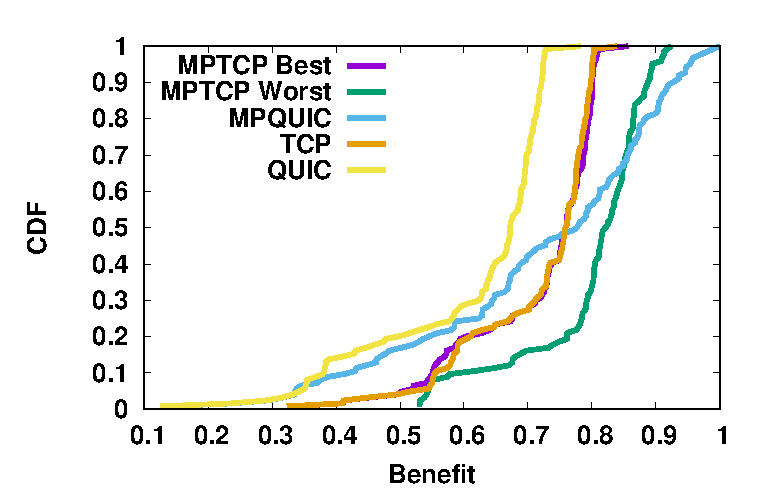
\includegraphics[width=.95\linewidth]{img/highbdp-lossless/highbdpnoloss_cdf.eps}
		 \caption{\label{fig:benefit-cdf-high} CDF of benefit of Viscous over other transport different protocol}
		\end{subfigure}
		\caption{\label{fig:benefit-high}Experimental results on lossless high BDP channels}
	\end{center}
\end{figure}


\begin{figure}
	\captionsetup[subfigure]{}
	\begin{center}
		\begin{subfigure}{.49\linewidth}
			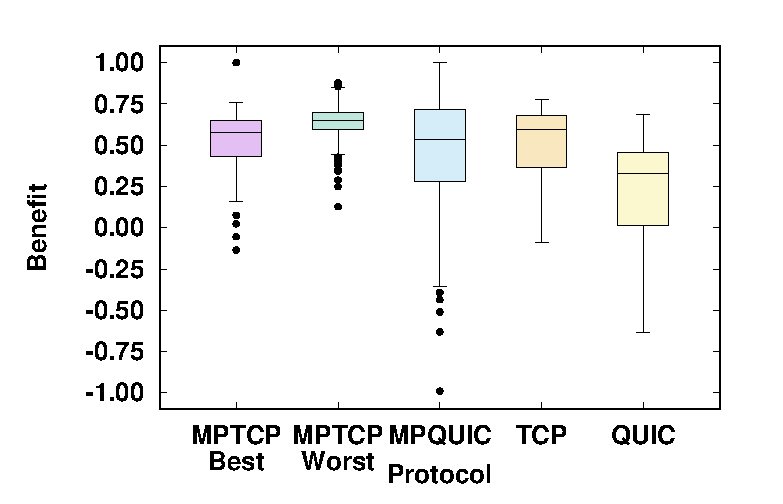
\includegraphics[width=.95\linewidth]{img/lowbdp-lossy/lowbdplossy_benefit.eps}
		 \caption{\label{fig:benefit-box-lossy} Benefit of Viscous over other transport different protocol}
		\end{subfigure}
		\begin{subfigure}{.49\linewidth}
			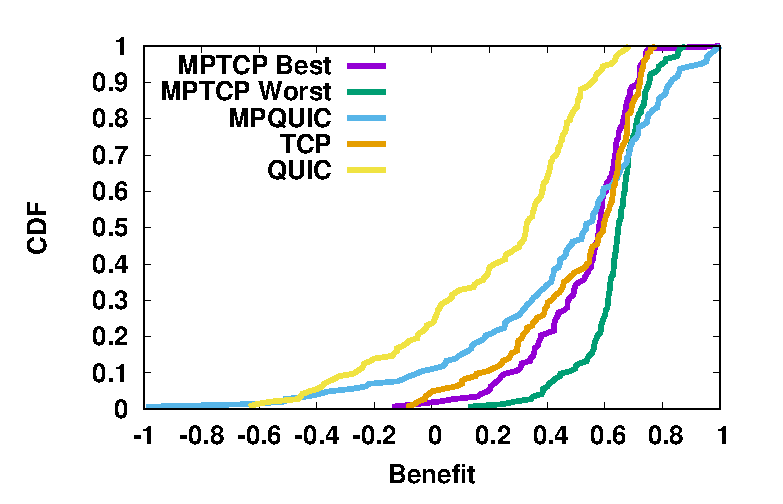
\includegraphics[width=.95\linewidth]{img/lowbdp-lossy/lowbdplossy_cdf.eps}
		 \caption{\label{fig:benefit-cdf-lossy} CDF of benefit of Viscous over other transport different protocol}
		\end{subfigure}
		\caption{\label{fig:benefit-lossy}Experimental results on lossy low BDP channels}
	\end{center}
\end{figure}

\begin{figure}
	\captionsetup[subfigure]{}
	\begin{center}
		\begin{subfigure}{.49\linewidth}
			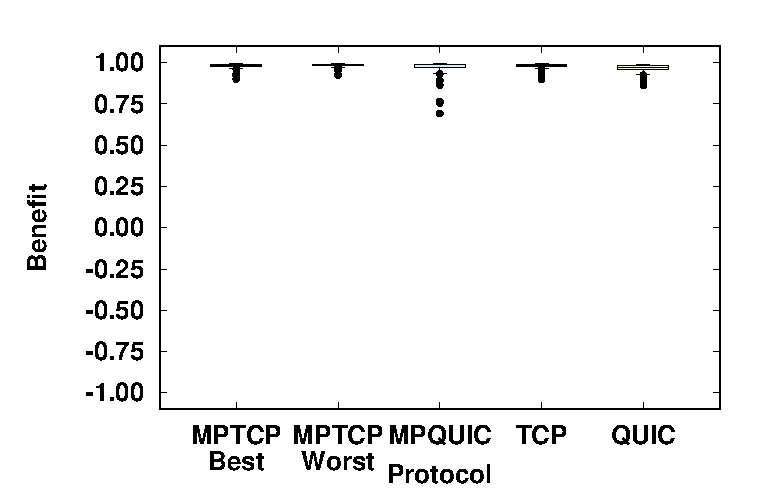
\includegraphics[width=.95\linewidth]{img/highbdp-lossy/highbdplossy_benefit.eps}
		 \caption{\label{fig:benefit-box-high-lossy} Benefit of Viscous over other transport different protocol}
		\end{subfigure}
		\begin{subfigure}{.49\linewidth}
			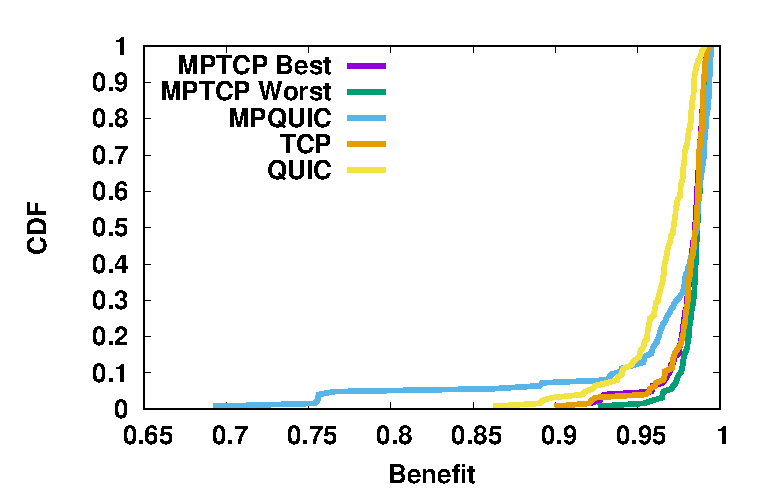
\includegraphics[width=.95\linewidth]{img/highbdp-lossy/highbdplossy_cdf.eps}
		 \caption{\label{fig:benefit-cdf-high-lossy} CDF of benefit of Viscous over other transport different protocol}
		\end{subfigure}
		\caption{\label{fig:benefit-high-lossy}Experimental results on lossy high BDP channels}
	\end{center}
\end{figure}


\begin{figure*}[h]
	\centering
	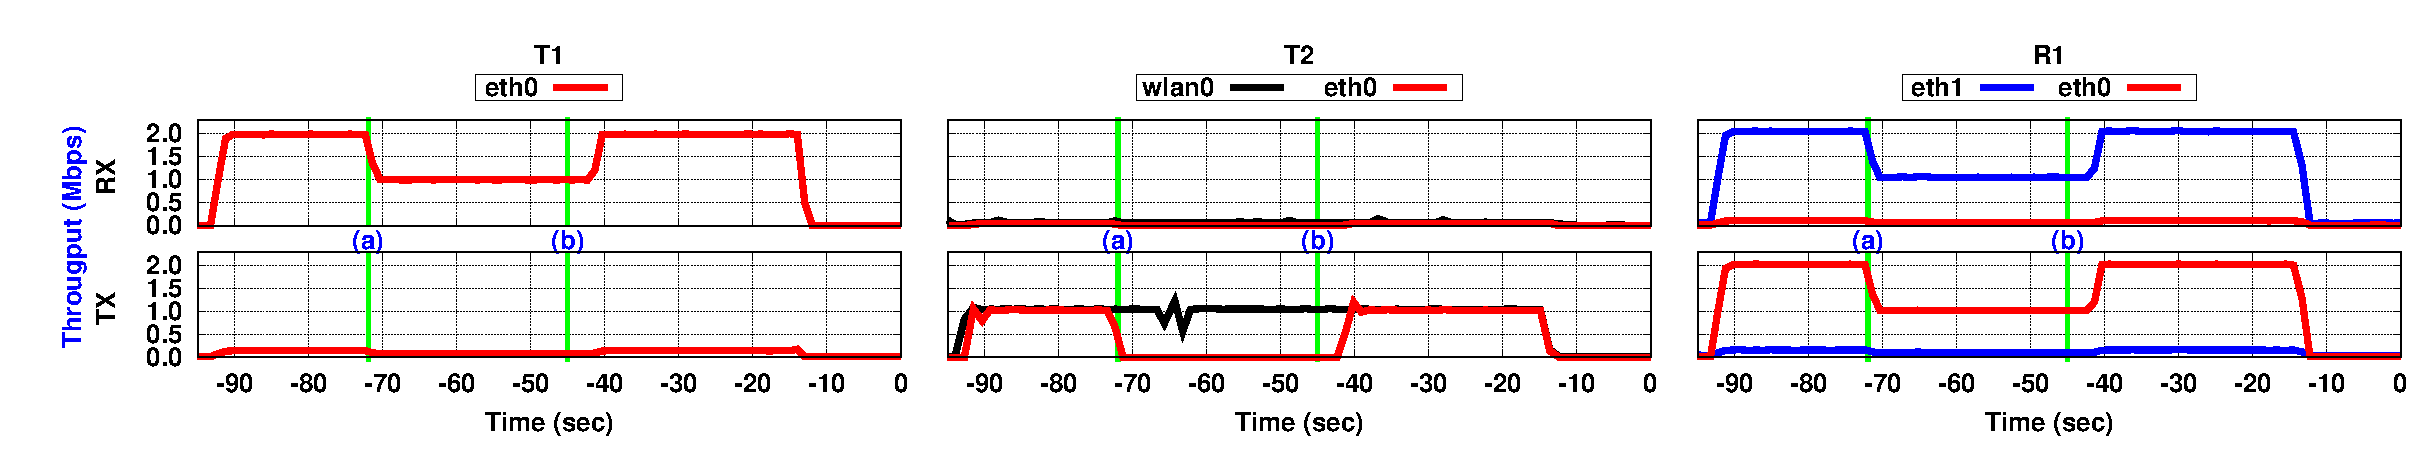
\includegraphics[width=\linewidth]{img/mobility/T1-T2-R1.eps}
	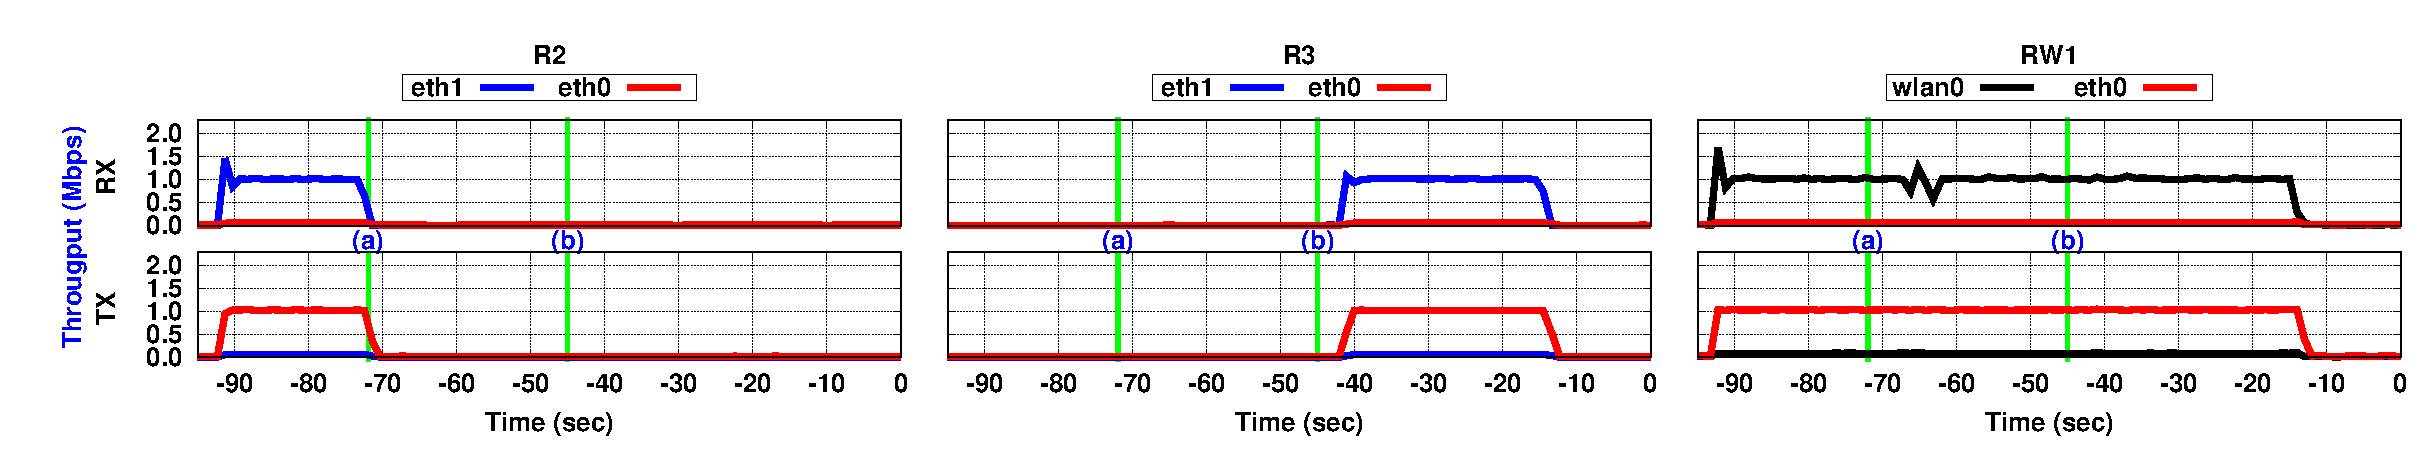
\includegraphics[width=\linewidth]{img/mobility/R2-R3-RW1.eps}
	\caption{\label{fig:mobility_res}RX-TX throughput at different hosts and routers}
\end{figure*}


\subsection{Mobility Support Analysis}

We have shown the result in Fig.~\ref{fig:mobility_res}. In these plots, we have depicted in-coming (RX) and out-going (TX) throughput for each network interfaces for two hosts and 4 routers two covering all the paths between T1 and T2. Top plots depict RX throughput over time and bottom plot depict TX throughput over time for each hosts and routers. Now, we disconnect the link between R4 and T2 at -65th seconds (marked as {\tt a} in plots) and we connect T2 with R3 at time -55 seconds (marked as {\tt b} in plots).

We can see that Viscous handles mobility pretty well. It easily detects the closed link and turn off data transmission through that link. It can also detect new link and establish a channel through the new link. We can see that it takes few seconds to establish a new connection. It is happening because we are using external tool NetworkManager to provided network connection-disconnection event to the Viscous for now.
